%%%%%%%%%%%%%%%%%%%%%%%%%%%%%%%%%%%%%%%%%%%%%%%%%%%%%%%%%%%
\subsection{Reflection and Transmission}
%%%%%%%%%%%%%%%%%%%%%%%%%%%%%%%%%%%%%%%%%%%%%%%%%%%%%%%%%%%

When light interacts with two materials that have different indexes of refraction, the incident beam is reflected and transmitted according to Fresnel’s equations.

The law of reflection states that the transmission angle of the reflected beam will be equal to the angle of the reflected beam in relation to the Z axis.
%
\begin{align}
    \theta_i = \theta_r
\end{align}
%
The transmission is derived directly from Snells equation,
%
\begin{align}
    n_1sin(\theta_1) = n_2sin(\theta_2)
\end{align}
%
% TODO: add snells equation graph here
Note that part of the transmitted spectra may be absorbed, although this is not considered in these equations.

Two main scenarios are often presented when demonstrating the principles which guide the reflected and transmitted rays; when the incident electromagnetic wave is polarized perpendicular to the plane of incidence, and when the wave is polarized parallel to it.  The perpendicular polarized wave is often denoted S or TE for transverse electric, while the parallel scenario is often denoted P or TM for transverse magnetic.

\begin{figure}[!htb]
    \begin{center}
        \makebox[\textwidth]{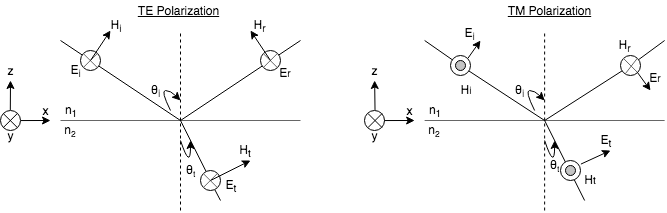
\includegraphics[scale=0.6]{/Sources/Background/Nature_of_Light/fresnel-reflect-trans.png}}
    \end{center}
    \caption{Fresnel Reflection and Transmittance}
    \label{fig:polarization}
\end{figure}

The intensity of the reflected waves for the S and P polarized case are
%
\begin{align}
    \mathbf{R_S} = |\frac{Z_2cos(\theta_i)-Z_1cos(\theta_t)}{Z_2cos(\theta_i)+Z_1cos(\theta_t)}|^2
\end{align}
\begin{align}
    \mathbf{R_P} = |\frac{Z_2cos(\theta_t)-Z_1cos(\theta_i)}{Z_2cos(\theta_t)+Z_1cos(\theta_i)}|^2
\end{align}
%
where Z is the wave impedance for medium 1 and 2.  The power coefficients for transmission are then derived by following the law of conservation of energy such that,
%
\begin{align}
    T_S = 1 - R_S \\
    T_P = 1 - R_P
\end{align}
%
The Brewster angle is a special case where the $P$ polarization state is completely transmitted and no reflection of the TM wave occurs.  The reflected ray is therefore completely $S$ polarized since $R_P$ is zero and $R_S$ is a nonzero intensity.  For perfect air glass interactions typically considered, this angle is approximately 55 degrees.

The Mueller matrix formulation for reflection and transmission reduces to the form of a linear polarizer for ideal surfaces.  It has been shown in \cite{polarizedlight} that the equation for a reflected beam off of a perfectly smooth dielectric surface is
%
\begin{align}
    \begin{split}
    \begin{bmatrix}
        S_{0r} \\
        S_{1r} \\
        S_{2r} \\
        S_{3r}
    \end{bmatrix}
    =
    \frac{1}{2}(\frac{tan(\theta_{-})}{sin(\theta_{+})})^2
    \begin{bmatrix}
       p_S^2 + p_P^2 & p_S^2 - p_P^2 & 0 & 0 \\
        p_S^2 - p_P^2 & p_S^2 + p_P^2 & 0 & 0 \\
        0 & 0 & 2p_Sp_P & 0 \\
        0 & 0 & 0 & 2p_Sp_P
    \end{bmatrix}
    \begin{bmatrix}
        S_0 \\
        S_1 \\
        S_2 \\
        S_3
    \end{bmatrix}
    \end{split}
\end{align}
%
\begin{align}
    p_S = cos^2(\theta_{-}) \\
    p_P = cos^2(\theta_{+})
\end{align}
and $\theta_{\pm}=\theta_i \pm \theta_r$.
This is identical to the form of a linear diattenuator or polarizer from Equation 2.60. For incident unpolarized light the equation simplifies to
%
\begin{align}
    \begin{bmatrix}
        S_{0r} \\
        S_{1r} \\
        S_{2r} \\
        S_{3r}
    \end{bmatrix}
    =
    \frac{1}{2}(\frac{tan(\theta_{-})}{sin(\theta_{+})})^2
    \begin{bmatrix}
        cos^2(\theta_{-}) + cos^2(\theta_{+}) \\
        cos^2(\theta_{-}) - cos^2(\theta_{+}) \\
        0 \\
        0
    \end{bmatrix}
    S_0
\end{align}
%
Therefore, for ideal reflective surfaces, at the Brewster angle, light will be completely polarized perpendicular to the plane of incidence. It should be noted that the case of incident unpolarized light onto the target material, gives the polarizance vector of the Mueller Matrix as described in Section 2.1.3.

Imperfect, non-ideal surfaces have the ability to reflect, transmit and absorb incident electromagnetic radiation.  The outcome of these interactions are related to the physiological makeup of the material, as well as its surface topology.  Multiple scattering mechanisms can be at work within a system, and numerous models have been attempted to balance the tradeoffs between practical realizability for measurements and accurate representation of scattering mechanisms \cite{priest}, \cite{pbrdf}.  Only some of these models attempt to deal with the polarization of the incident, reflected, and transmitted beams.
